\documentclass[a4paper,12pt]{article}
\usepackage[T1]{fontenc}
\usepackage[utf8]{inputenc}
\usepackage{lmodern}
\usepackage[spanish]{babel}
\usepackage{textcomp}
\usepackage{amsmath}
\usepackage{amsfonts}
\usepackage[framed,numbered,autolinebreaks]{mcode}
\usepackage{amssymb}
\usepackage{graphicx}
\usepackage{caption}
\usepackage{subcaption}
\usepackage{float}
\usepackage{color}
\usepackage{multicol}
\usepackage{mcode}
\usepackage[left=2cm,right=2cm,top=2cm,bottom=2cm]{geometry}
\usepackage{fancyhdr}
\usepackage[hidelinks]{hyperref}
\title{Serie-Examen}
\author{
  Cabrera López Oscar Emilio
}

\pagestyle{fancy}
\fancyhf{}
\lhead[]{}
\chead[]{}
\rfoot{\thepage}
\lfoot[]{}
\cfoot[]{}

\linespread{1.3}

\renewcommand\headrule
{{\color[RGB]{98,36,35}%
    \hrule height 2pt
    width\headwidth
    \vspace{1.3pt}%
    \hrule height 1pt
    width\headwidth
  }}
  \addto\captionsspanish{\def\tablename{Tabla}}%imprime Tabla en lugar de Cuadro
  %%
  \spanishdecimal{.}


\begin{document}
\thispagestyle{fancy}
\maketitle
\newpage
\tableofcontents
\newpage

\section{Ejercicio 1}
Si la respuesta al impulso es:
\[ h[n] =\left((n +1) \left(\frac{1}{5}\right)^{n-1}\right)u[n] \]
\begin{itemize}
    \item[a)] Obtenga $H(z)$ y diga si es o no estable el sistema.
            \[ \mathcal{Z}\left\{h[n] = n\left(\frac{1}{5}\right)^{n-1}u[n] + \left(\frac{1}{5}\right)^{n-1}u[n]\right\} \]
            \[ H(z) = \frac{z^{-1}}{(1-\frac{1}{5}z^{-1})^2} + \frac{5}{1-\frac{1}{5}z^{-1}} \]
        la función de transferencia en el dominio de $Z$ es:
            \[ H(z) = \frac{5}{(1-\frac{1}{5}z^{-1})^2} \]
        dado que los polos y los ceros del sistema son reales y menores a 1, se encuentran dentro del círculo unitario por lo tanto este sistema es estable.
    \item[b)] Determine el diagrama de bloques del sistema
        \[ Y(z) = -\frac{1}{25}z^{-2}Y(z) + \frac{2}{5}z^{-1}Y(z) + 5X(z) \]
        \begin{figure}[H]
            \begin{center}
                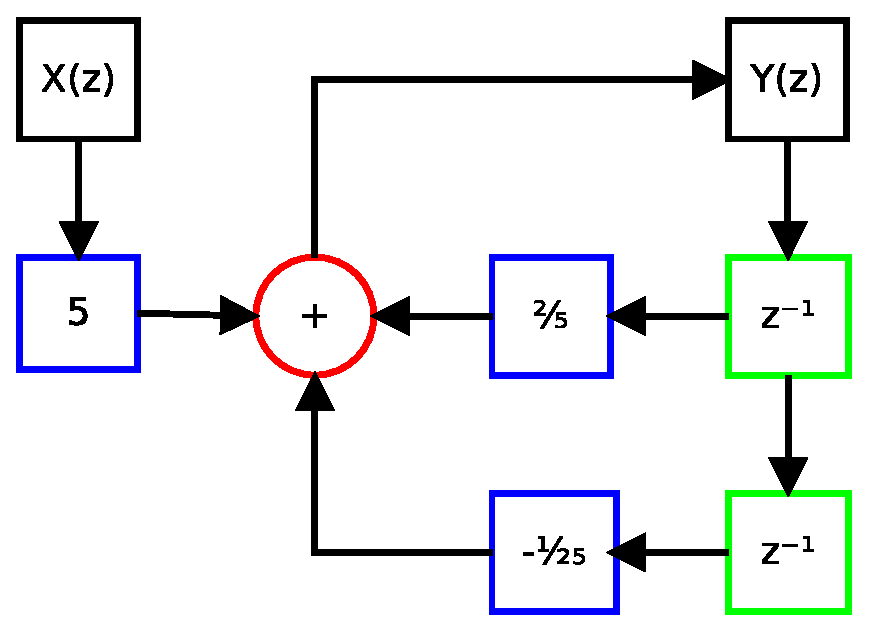
\includegraphics[width=0.8\linewidth]{Diagrama}
                \caption{Diagrama de bloques del sistema}
                \label{fig:dia1}
            \end{center}
        \end{figure}
    \item[c)] Obtenga los primeros 5 valores de $h[n]$ mediante recursividad.
        \[ \begin{split}
            x[n] &= \delta[n]\\
            y[n] &= -\frac{1}{25}y[n-2] + \frac{2}{5}y[n-1] + 5x[n]\\
            y[0] &= 5\\
            y[1] &= \frac{2}{5}(5) = 2 \\
            y[2] &= -\frac{1}{25}(5) + \frac{2}{5}(2) = \frac{3}{5}\\
            y[3] &= -\frac{1}{25}\left(2\right) + \frac{2}{5}\left(\frac{3}{5}\right) = \frac{4}{25} \\
            y[4] &= -\frac{1}{25}\left(\frac{3}{5}\right) + \frac{2}{5}\left(\frac{4}{25}\right) = \frac{1}{25} \\
            y[5] &= -\frac{1}{25}\left(\frac{4}{25}\right) + \frac{2}{5}\left(\frac{1}{25}\right) = \frac{6}{625} \\
        \end{split} \]
    \item[d)] Obtenga la respuesta al escalón mediante convolución.
        \[ \begin{split}
            x[n] &= u[n] \\
            y[n] &= h[n] \ast u[n] \\
            y[n] &= \sum_{k=-\infty}^{\infty}\left((k + 1)\left(\frac{1}{5}\right)^{k-1}\right)u[k]u[n - k] \\&
            u[n] =\begin{cases}
                 1 & k \geq 0 \\
                 0 & k < 0
                 \end{cases} \qquad
            u[n] =\begin{cases}
                 1 & k \leq n \\
                 0 & k > n
                 \end{cases} \\
            y[n] &= \sum_{k=0}^{n}\left(k\left(\frac{1}{5}\right)^{k-1} +  \left(\frac{1}{5}\right)^{k-1}\right) \\
            y[n] &= 5\sum_{k=1}^{n}k\left(\frac{1}{5}\right)^k + 5\sum_{k=0}^{n}\left(\frac{1}{5}\right)^k \\
            y[n] &= 5\sum_{k=1}^{n}k\left(\frac{1}{5}\right)^k + 5\sum_{k=0}^{n}\left(\frac{1}{5}\right)^k \\
            y[n] &= 5\left( \frac{\frac{1}{5}}{\left(1-\frac{1}{5}\right)} \left( 1 - (n+1)\left(\frac{1}{5}\right)^n + n\left(\frac{1}{5}\right)^{n + 1} \right) + \frac{1-\left(\frac{1}{5}\right)^{n + 1}}{1 - \frac{1}{5}} \right)u[n]
        \end{split} \]
\end{itemize}\newpage
\section{Ejercicio 2}
Para el sistema de tiempo discreto, establecido mediante el diagrama de polos y ceros, con ganancia 2:
\begin{figure}[H]
    \begin{center}
        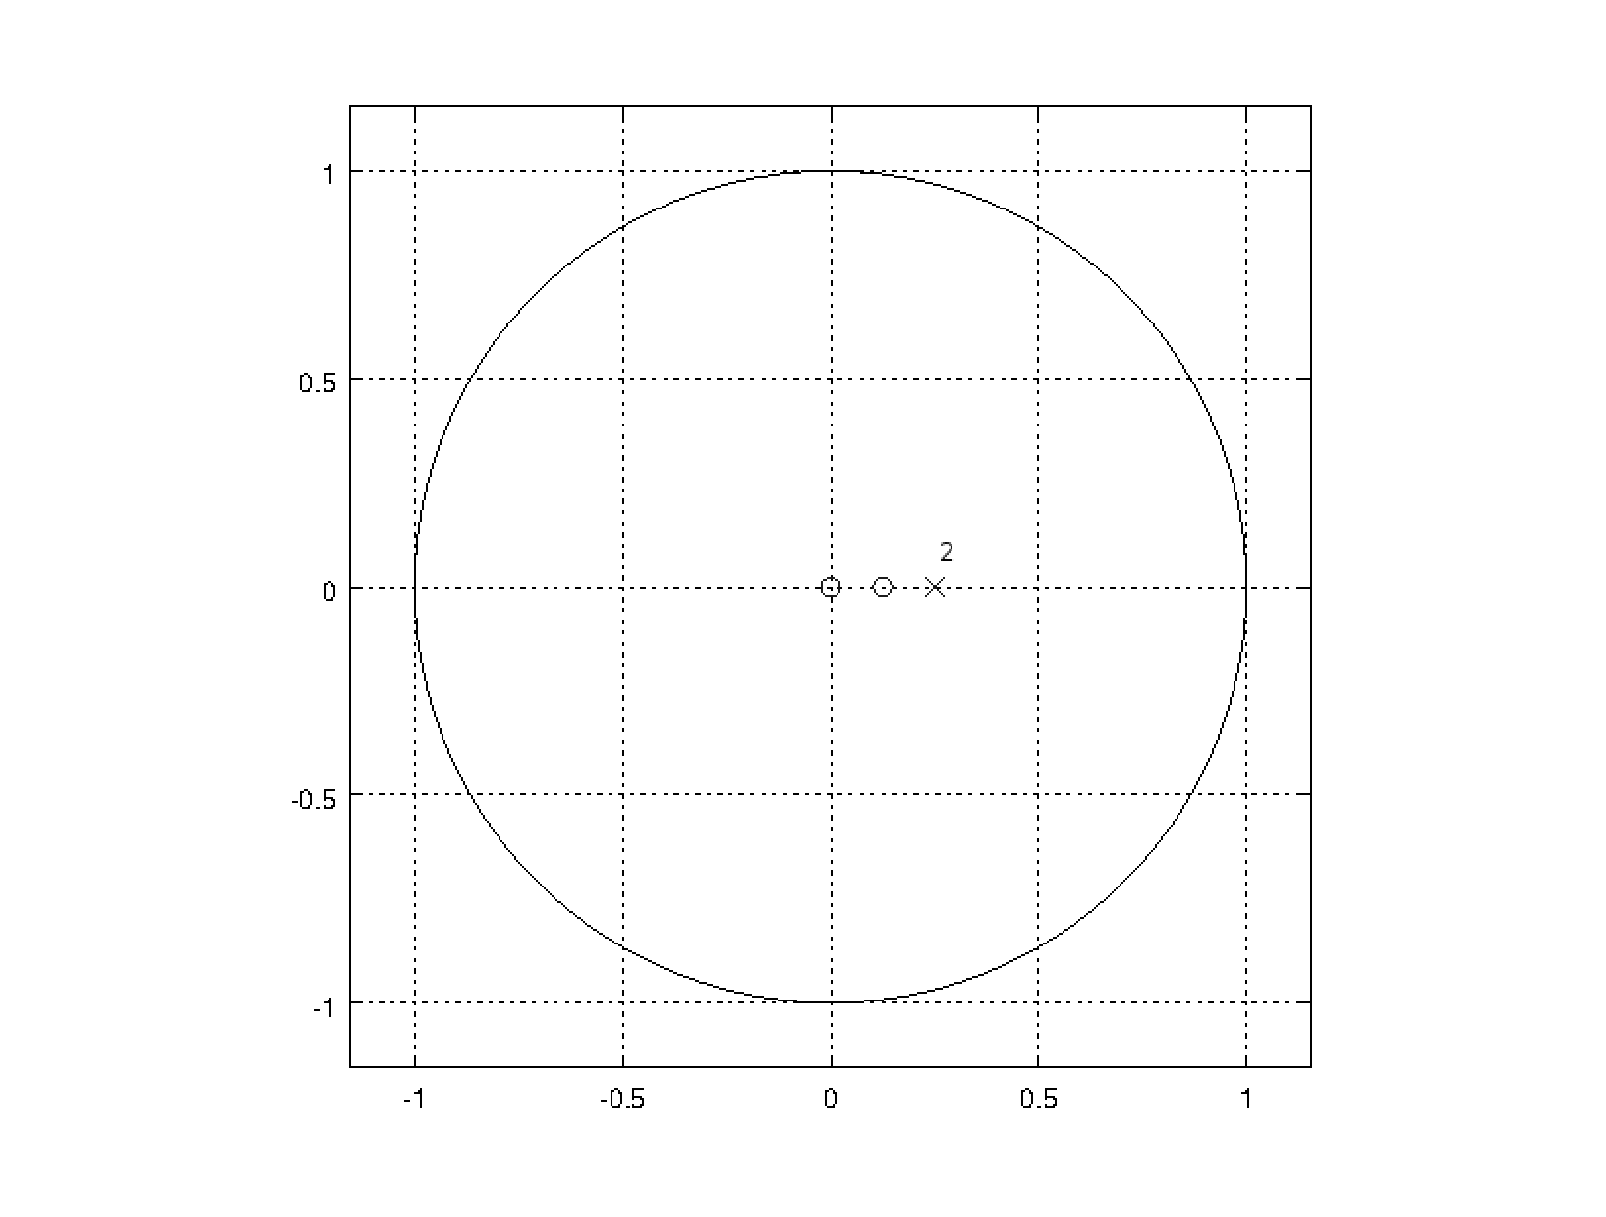
\includegraphics[width=0.7\linewidth]{polosZeros1.eps}
        \caption{Diagrama de polos y ceros del sistema}
        \label{fig:polosZeros1}
    \end{center}
\end{figure}
\begin{itemize}
    \item[a)] Determine la función de transferencia. \\
        En la figura vemos que el numerador es un polinomio $X(z)$ con una raíz en $z = \frac{1}{8}$ y otra en $z = 0$ mientras que el denominador es un polinomio $Y(z)$ con dos raíces en $z = \frac{1}{4}$ entonces la función de transferencia es:
        \[ H(z) = \frac{2z\left(z - \frac{1}{8}\right)}{\left(z - \frac{1}{4}\right)^2} \]
        Comprobando con Matlab:
        \begin{lstlisting}
>> sysz = zpk([0 1/8],[1/4 1/4],2,1)
Transfer function 'sysz' from input 'u1' to output ...

         2 z^2 - 0.25 z
 y1:  --------------------
      z^2 - 0.5 z + 0.0625

Sampling time: 1 s
Discrete-time model.
        \end{lstlisting}
    \item[b)] La respuesta al impulso. \\
        Operamos, descomponemos en fracciones parciales y anti-transformamos:
        \[ H(z) = \frac{2z^2 - \frac{1}{4}z}{z^2 - \frac{1}{2}z + \frac{1}{16}}\frac{z^{-2}}{z^{-2}} = \frac{2 - \frac{1}{4}z^{-1}}{\left(1-\frac{1}{4}z^{-1}\right)^2} = \frac{1}{\left(1-\frac{1}{4}z^{-1}\right)} + \frac{1}{\left(1-\frac{1}{4}z^{-1}\right)^2} \]
        \[ \mathcal{Z}^{-1}\left\{H(z) = \frac{1}{\left(1-\frac{1}{4}z^{-1}\right)} + z\frac{z^{-1}}{\left(1-\frac{1}{4}z^{-1}\right)^2}\right\} \]
        \[ h[n] = \left(\frac{1}{4}\right)^n u[n] + (n+1)\left(\frac{1}{4}\right)^n u[n+1] \]
    \item[c)] La respuesta al escalón. \\
        Multiplicamos por la transformada $Z$ del escalón, operamos, descomponemos en fracciones parciales y anti-transformamos:
        \[ H(z) = \frac{2z^2 - \frac{1}{4}z}{\left(z^2 - \frac{1}{4}\right)^2}\frac{z}{z-1} \]
        \[ \frac{H(z)}{z} = \frac{2z^2 - \frac{1}{4}z}{\left(z^2 - \frac{1}{4}\right)^2\left(z-1\right)} = \frac{-\frac{7}{9}}{z-\frac{1}{4}} + \frac{-\frac{1}{3}}{\left(z-\frac{1}{4}\right)^2} + \frac{\frac{28}{9}}{z-1} \]
        \[ \mathcal{Z}^{-1}\left\{ H(z) = -\frac{7}{9}\frac{z}{z-\frac{1}{4}} - \frac{1}{3}\frac{z}{\left(z-\frac{1}{4}\right)^2} + \frac{28}{9}\frac{z}{z-1} \right\} \]
        \[ h[n] = \left( \frac{28}{9} - \frac{7}{9}\left(\frac{1}{4}\right)^n - \frac{1}{3}n\left(\frac{1}{4}\right)^{n-1}\right)u[n] \]
    \item[d)] El diagrama de bloques.
        \[ Y(z) = \frac{1}{2}z^{-1}Y(z) - \frac{1}{16}z^{-2}Y(z) + 2X(z) - \frac{1}{4}z^{-1}X(z) \]
        \begin{figure}[H]
            \begin{center}
                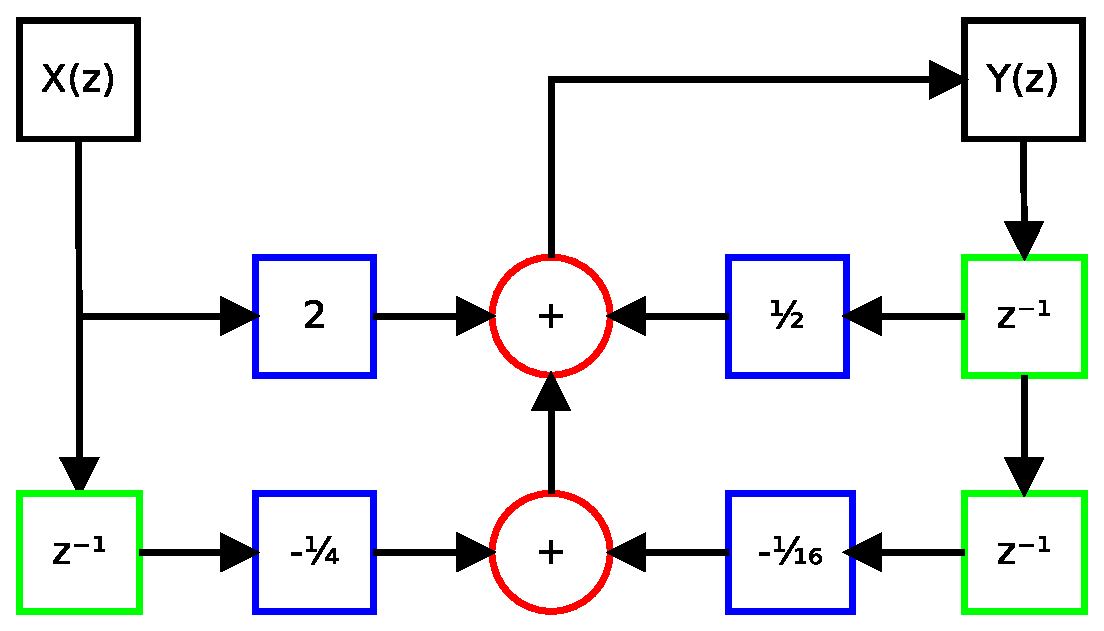
\includegraphics[width=0.6\linewidth]{Diagrama2}
                \caption{Diagrama de bloques del sistema}
                \label{fig:Dia1}
            \end{center}
        \end{figure}
\end{itemize}
\section{Ejercicio 3}
Los coeficientes de la serie de Fourier de una señal x(t) periódica con periodo T=8 son los siguientes:
\[ a_k =\begin{cases}
            2, & k = 0 \\
            \left(\frac{1}{2}\right)^{|k|}, & k \neq 0
        \end{cases}
 \]
    \begin{itemize}
        \item[a)] Grafique el espectro discreto de x(t).
        \begin{multicols}{2}
            \begin{figure}[H]
                \begin{center}
                    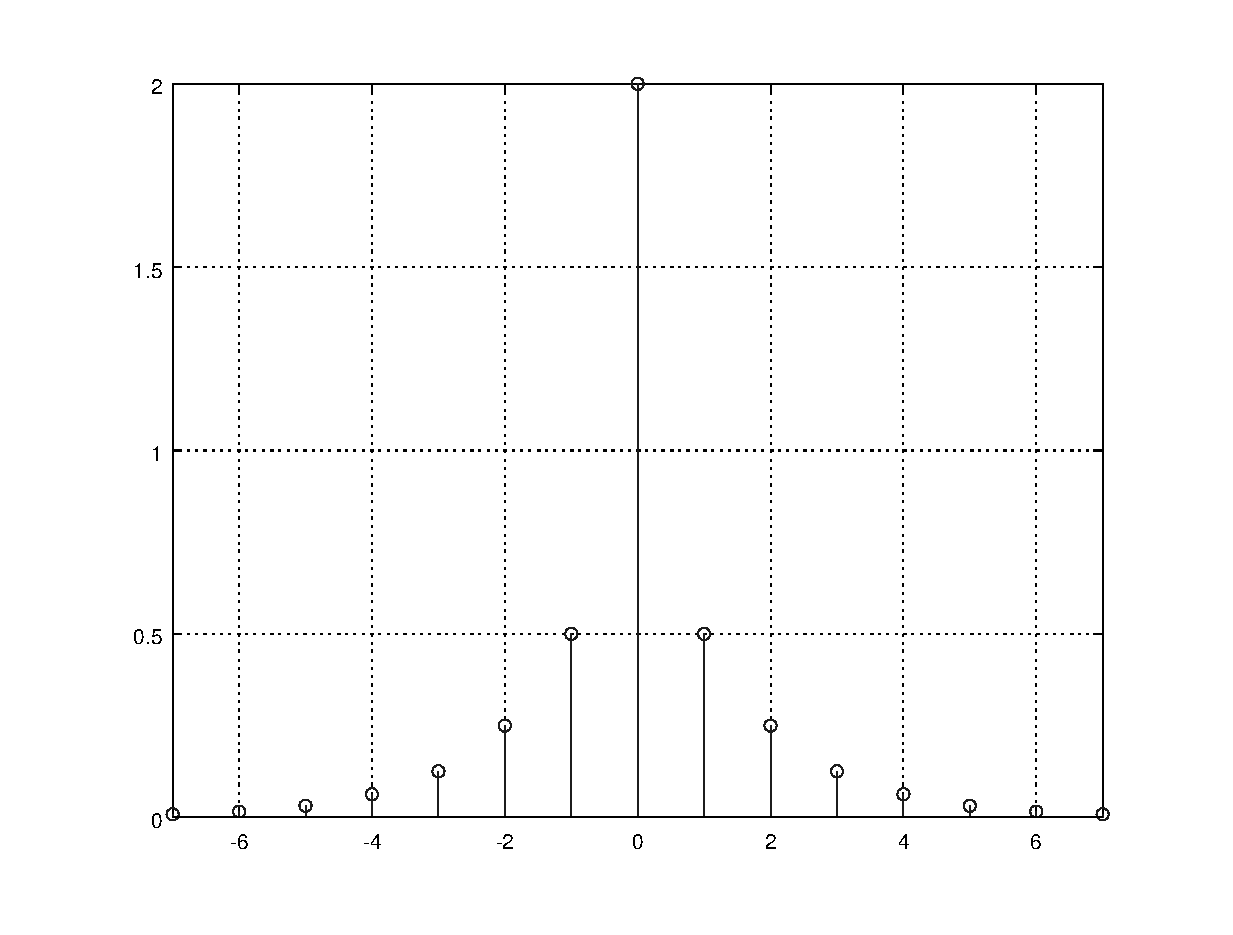
\includegraphics[width=\linewidth]{espectro1}
                    \caption{Gráfica del espectro de frecuencias}
                    \label{fig:espectro1}
                \end{center}
            \end{figure}
        \columnbreak
        Código en Matlab:
        \lstinputlisting{ak.m}
            \begin{lstlisting}
k = -7:7;
stem(k,ak(k));
axis([-7 7 0 2]);grid;
            \end{lstlisting}
        \end{multicols}
        
        \item[b)] Obtenga y grafique la señal $x(t)$.
        \[ \omega = \frac{2\pi}{T} = \frac{2\pi}{8} = \frac{\pi}{4} \]
        \[ x(t) = \underbrace{2}_{k=0} + 
                    \underbrace{cos\left(\frac{\pi}{4}t\right)}_{k=1} + 
                    \underbrace{\left(\frac{1}{2}\right)cos\left(\frac{\pi}{2}t\right)}_{k=2} +
                    \underbrace{\left(\frac{1}{4}\right)cos\left(\frac{3\pi}{4}t\right)}_{k=3} + 
                    \underbrace{\left(\frac{1}{8}\right)cos\left(\pi t\right)}_{k=4} + \cdots \]
        \[ x(t) = 2 + 2\sum_{k=1}^{\infty}\left(\frac{1}{2}\right)^{|k|}cos\left(\frac{k\pi}{4}t\right) \]
        \begin{multicols}{2}
            \begin{figure}[H]
                \begin{center}
                    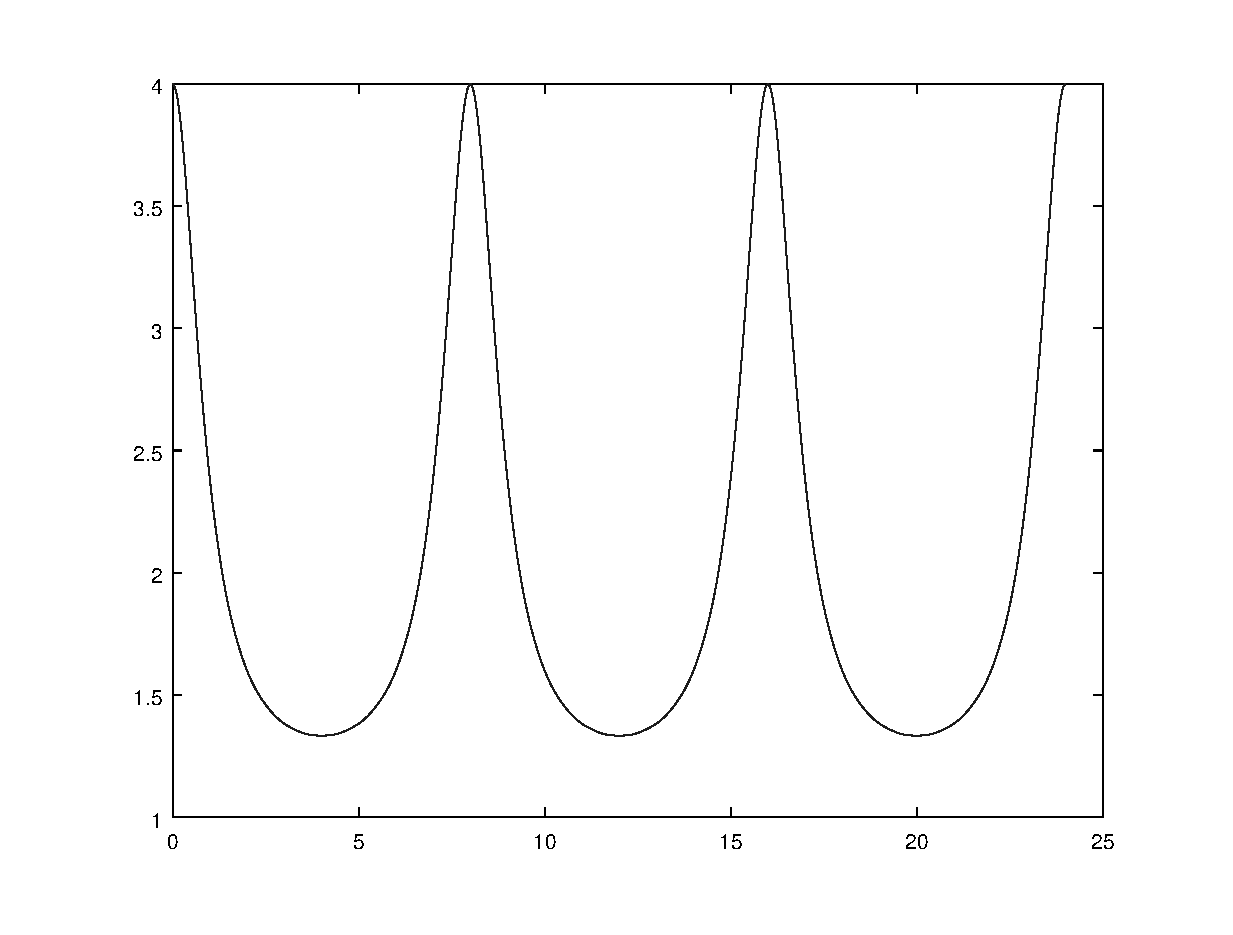
\includegraphics[width=\linewidth]{x1}
                    \caption{Gráfica de la señal a partir de sus coeficientes espectrales}
                    \label{fig:x1}
                \end{center}
            \end{figure}
        \columnbreak
        Código en Matlab:
        \lstinputlisting{x1.m}
            \begin{lstlisting}
t = 0:0.01:8*3;
plot(t,x1(10,t));
            \end{lstlisting}
        \end{multicols}
        \item[c)] Filtre la señal $x(t)$ a través de un filtro Butterworth de manera que elimine la
componente de directa y la primera armónica. \\
        Necesitamos un filtro que elimine las frecuencias menores a $\frac{\pi}{2}$, esto es un filtro paso-altas, una frecuencia de corte adecuada para este filtro es $\omega_c=\frac{3\pi}{8}$
        \begin{figure}[H]
            \begin{center}
                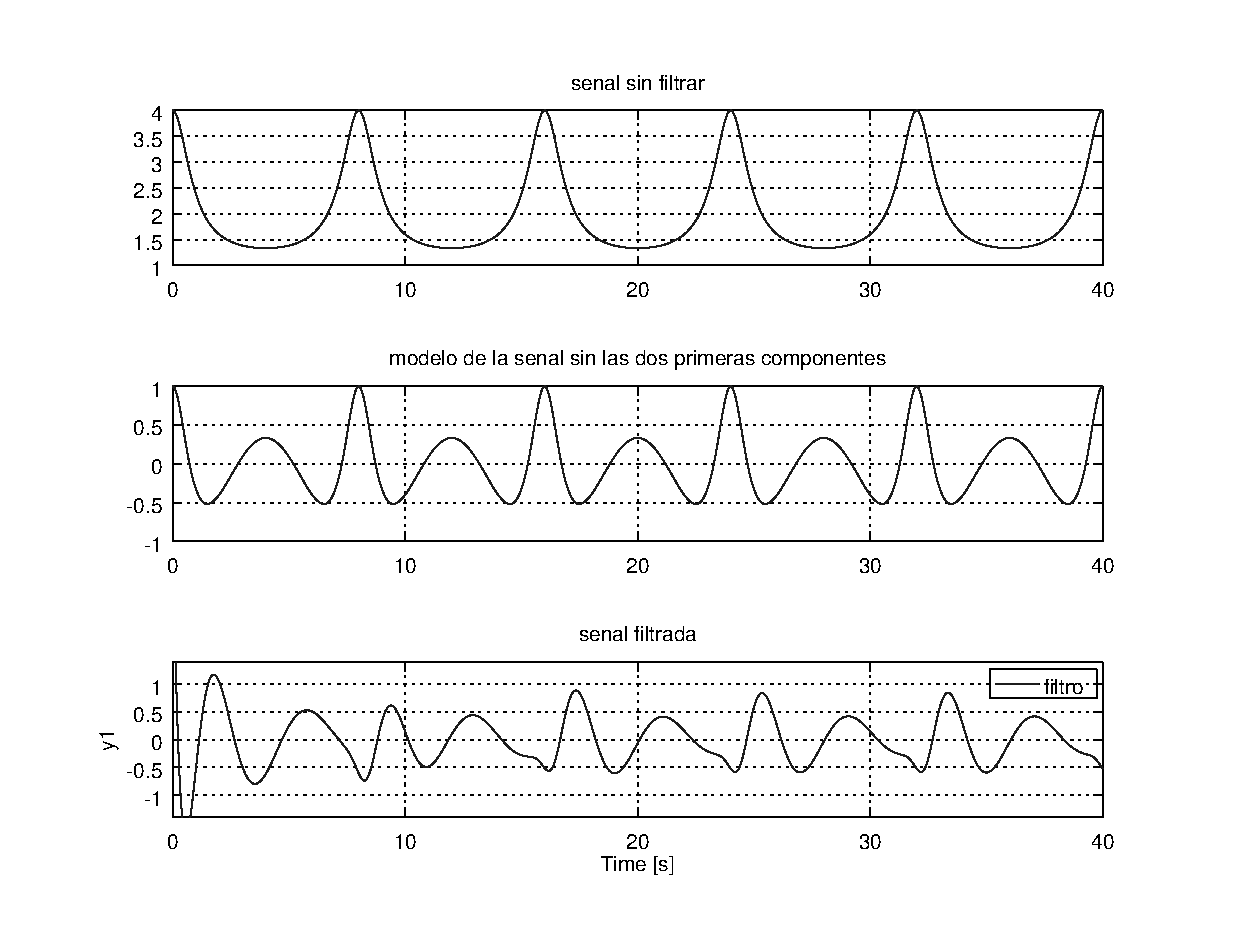
\includegraphics[width=\linewidth]{signalFiltrada}
                \caption{Gráficas de la señal filtrada}
                \label{fig:signalFil}
            \end{center}
        \end{figure}
        Código en Matlab:
        \lstinputlisting{filtro1.m} \newpage
        \item[d)] Presente el modelo del filtro seleccionado.
        \[ H(s) = \frac{s^8}{s^8 + \frac{4366}{723}s^7 + \frac{8369}{459}s^6 + \frac{25183}{705}s^5 + \frac{1543}{304}s^4 + \frac{31531}{636}s^3 + \frac{14049}{400}s^2 + \frac{13158}{815}s^1 + \frac{3347}{902}} \]
        \begin{lstlisting}
[b a] = butter(8,3*pi/8,'high','s');
filtro = tf(b,a)
        \end{lstlisting}
        \item[e)] Grafique la respuesta en frecuencia, en magnitud y fase, del filtro seleccionado.
        \begin{figure}[H]
            \begin{center}
                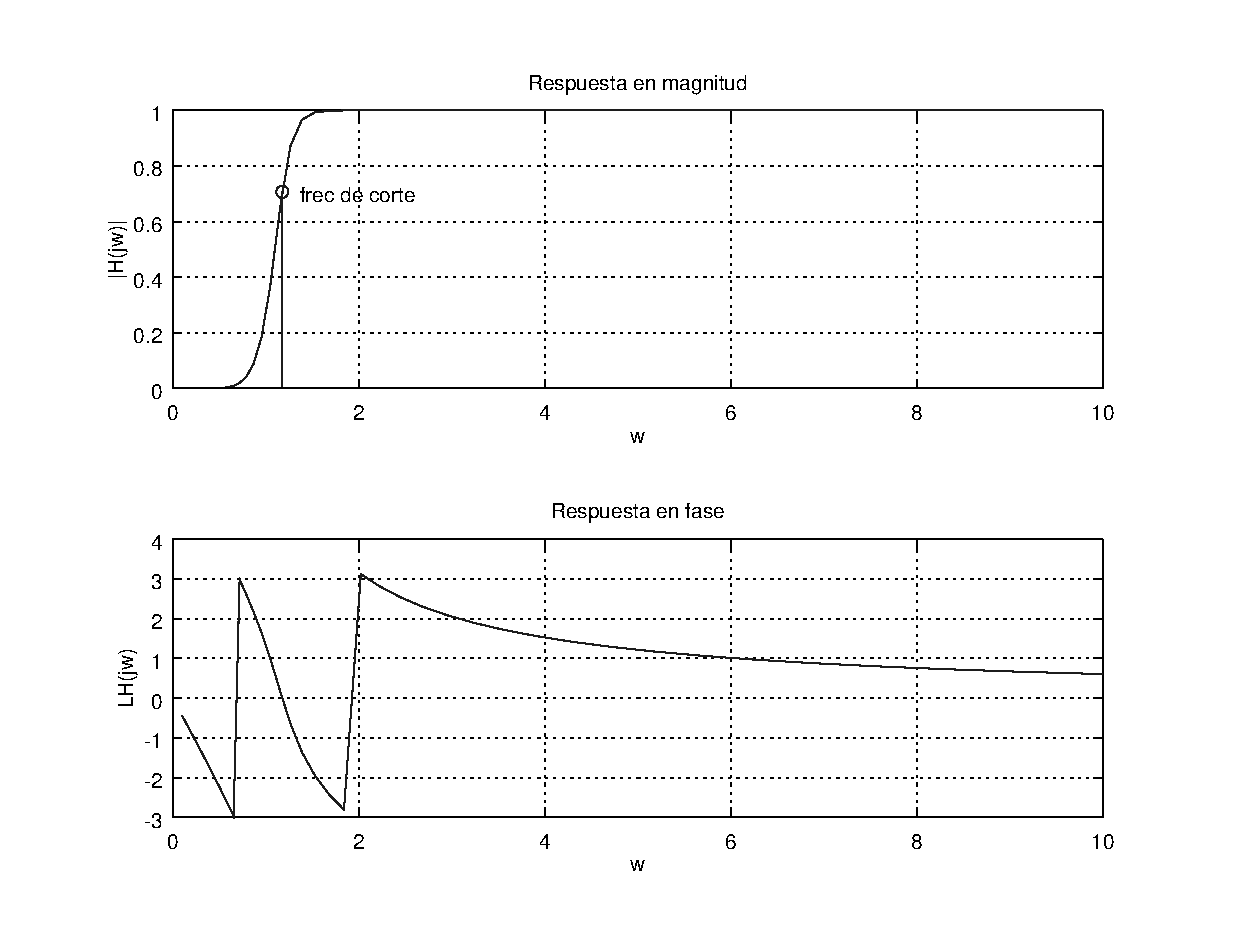
\includegraphics[width=\linewidth]{modeloFiltro.eps}
                \caption{Respuestas del filtro}
                \label{fig:respFil}
            \end{center}
        \end{figure}
        \lstinputlisting{modeloFiltro.m}
    \end{itemize}
\section{Ejercicio 4}
Una señal $x[n]$ periódica está definida como:
\[ x[n]=\begin{cases}
            1 & 0 \leq n \leq 4 \quad;\quad 6 \leq n \leq 9 \\
            0 & n = 5
        \end{cases}
 \]
y el periodo es de 10.
\begin{itemize}
    \item[a)] Determine y grafique los coeficientes de la serie de Fourier.
        \[ \begin{split}
            \omega &= \frac{2\pi}{10} = \frac{\pi}{5} \\
            a_0 &= \frac{1}{10}\sum_{n = -4}^{4}1 = \frac{9}{10} \qquad a_k = \underbrace{\frac{1}{10}\sum_{n=-4}^{4}e^{-jk\frac{\pi}{5}n}}_{m = n + 4} \\
            a_k &= \frac{1}{10}\sum_{m=0}^{8}e^{-jk\frac{\pi}{5}(m - 4)} = \frac{e^{jk\frac{4\pi}{5}}}{10}\sum_{m=0}^{8}e^{-jk\frac{\pi}{5}m} \\
            a_k &= \frac{e^{jk\frac{4\pi}{5}}}{10}\left(\frac{1 - e^{-jk\frac{9\pi}{5}}}{1 - e^{-jk\frac{\pi}{5}}}\right) = \frac{e^{jk\frac{4\pi}{5}}}{10}\left(- e^{jk\frac{\pi}{5}}\right) = -\frac{e^{jk\left(\frac{4\pi}{5} + \frac{\pi}{5}\right)}}{10} \\
            a_k &= -\frac{e^{jk\pi}}{10} \quad a_1 = -\frac{e^{jk\pi}}{10} \quad a_2 = -\frac{e^{j2\pi}}{10} \quad a_3 = -\frac{e^{j3\pi}}{10} \\
            a_4 &= -\frac{e^{j4\pi}}{10} \quad a_5 = -\frac{e^{j5\pi}}{10} \quad a_6 = -\frac{e^{j6\pi}}{10} \quad a_7 = -\frac{e^{j7\pi}}{10} \\
            a_8 &= -\frac{e^{j8\pi}}{10} \quad a_9 = -\frac{e^{j9\pi}}{10}
        \end{split} \]
        \begin{multicols}{2}
            \begin{figure}[H]
                \begin{center}
                    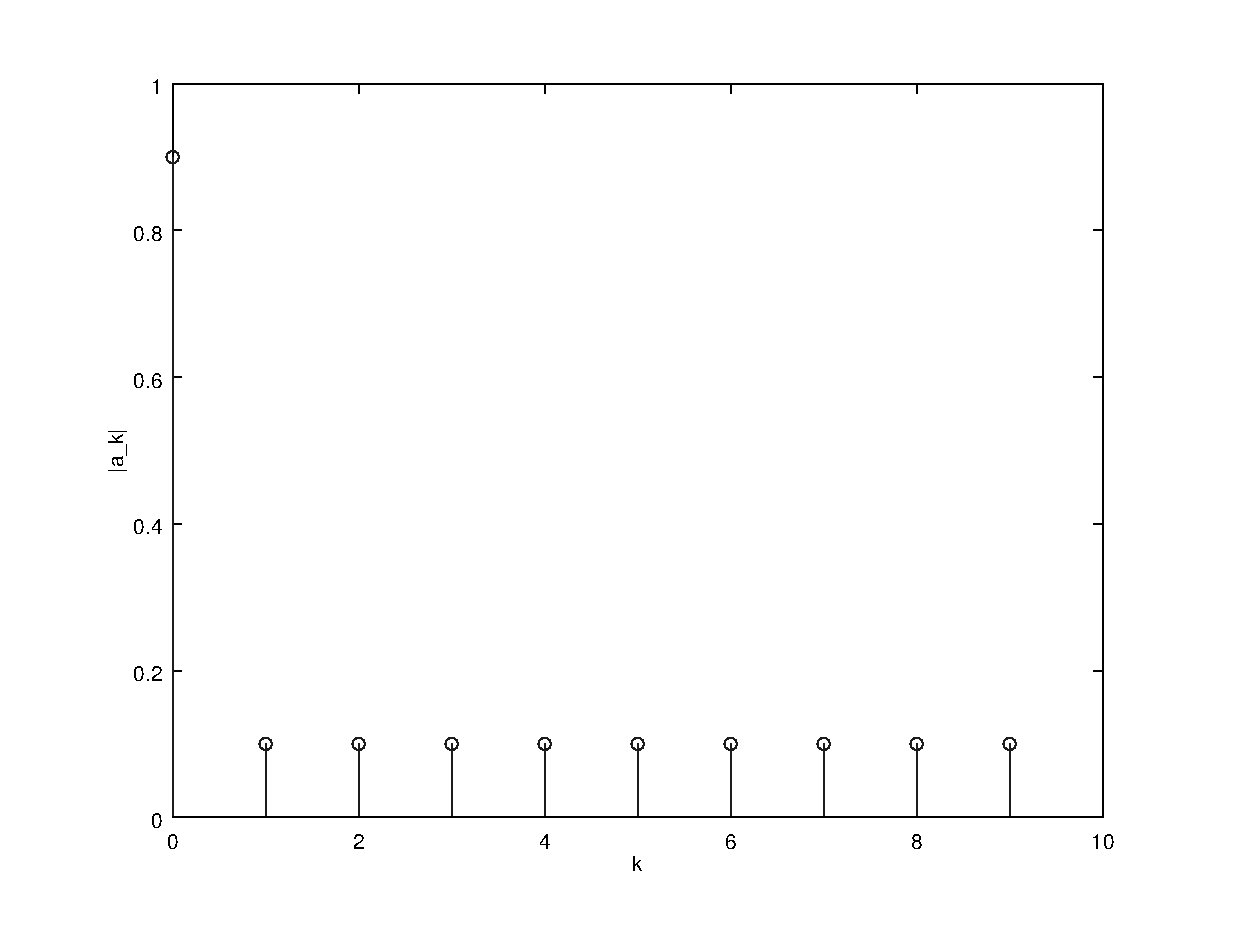
\includegraphics[width= \linewidth]{absAk}
                    \caption{Magnitud de los coeficientes espectrales}
                    \label{fig:absAk}
                \end{center}
            \end{figure}
            \columnbreak
            \begin{figure}[H]
                \begin{center}
                    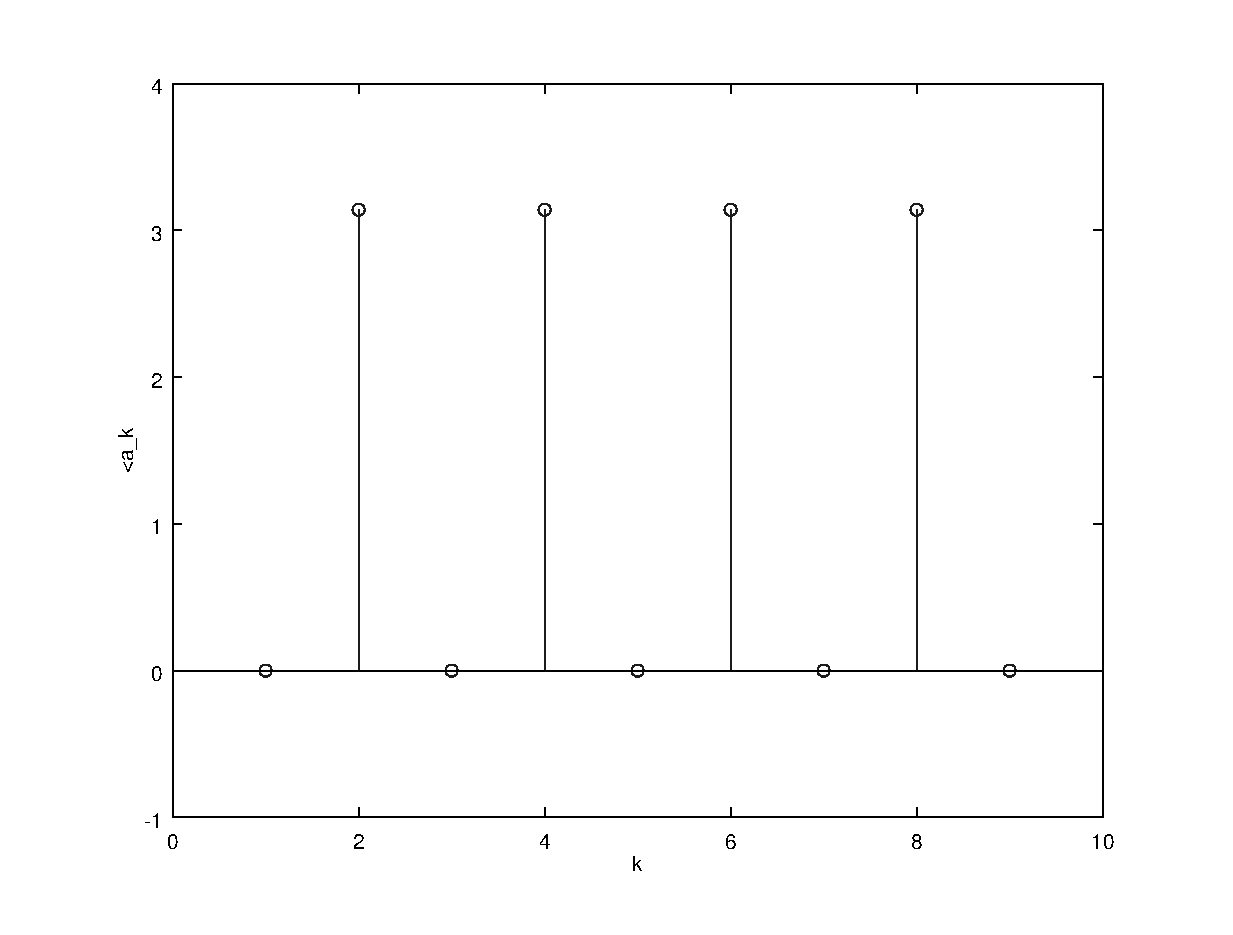
\includegraphics[width= \linewidth]{angleAk}
                    \caption{Fase de los coeficientes espectrales}
                    \label{fig:angleAk}
                \end{center}
            \end{figure}
        \end{multicols}
    \item[b)] A partir de los coeficientes obtenga de nuevo la señal.
    \[ x[n] = \frac{9}{10} -\frac{1}{10} \sum_{k = 1}^{9} e^{jk\frac{\pi}{5}n} e^{jk\pi} = \frac{9}{10} -\frac{1}{10} \sum_{k = 1}^{9} e^{jk(\frac{\pi}{5}n + \pi)} \]
\end{itemize}
\section{Ejercicio 5}
Considere las señales $x(t)$ y $x1(t)$.
\begin{multicols}{2}
    \begin{figure}[H]
        \begin{center}
            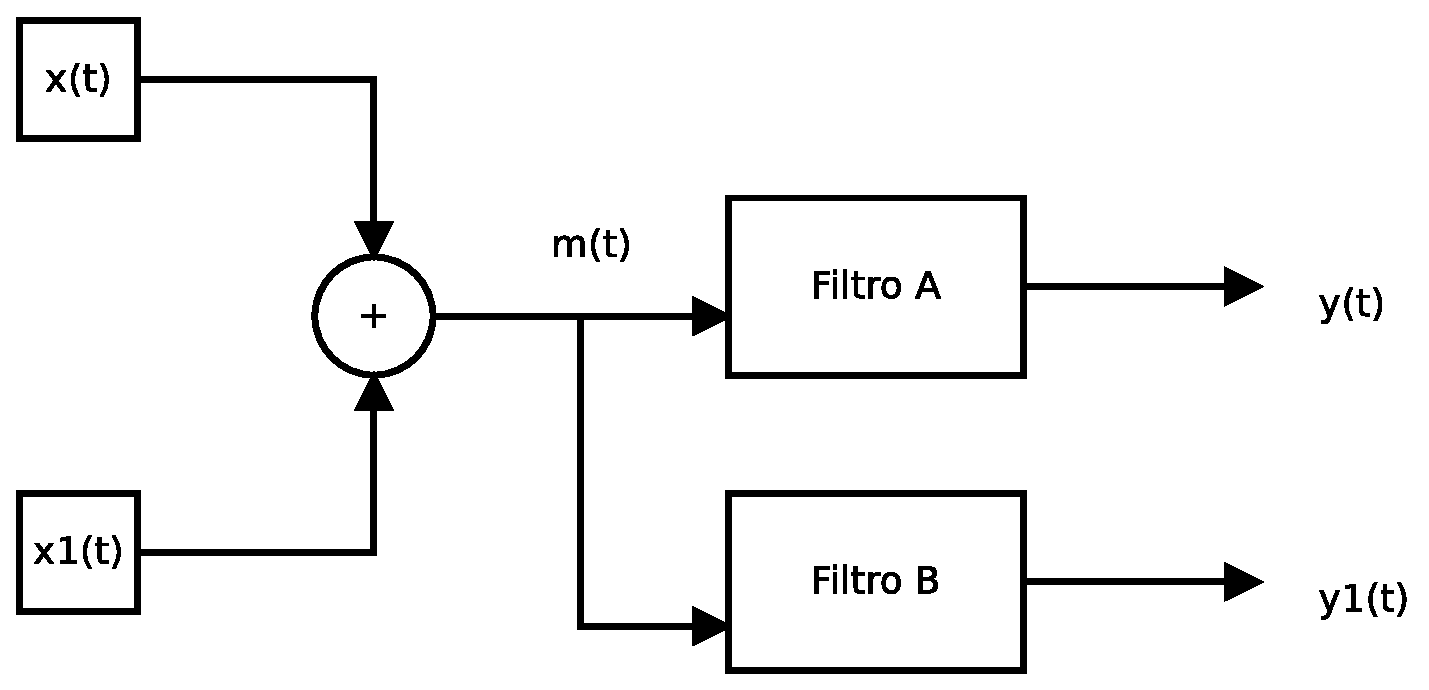
\includegraphics[width=\linewidth]{Diagrama3}
            \label{fig:Dia3}
        \end{center}
    \end{figure}
    \columnbreak
    \begin{figure}[H]
        \begin{center}
            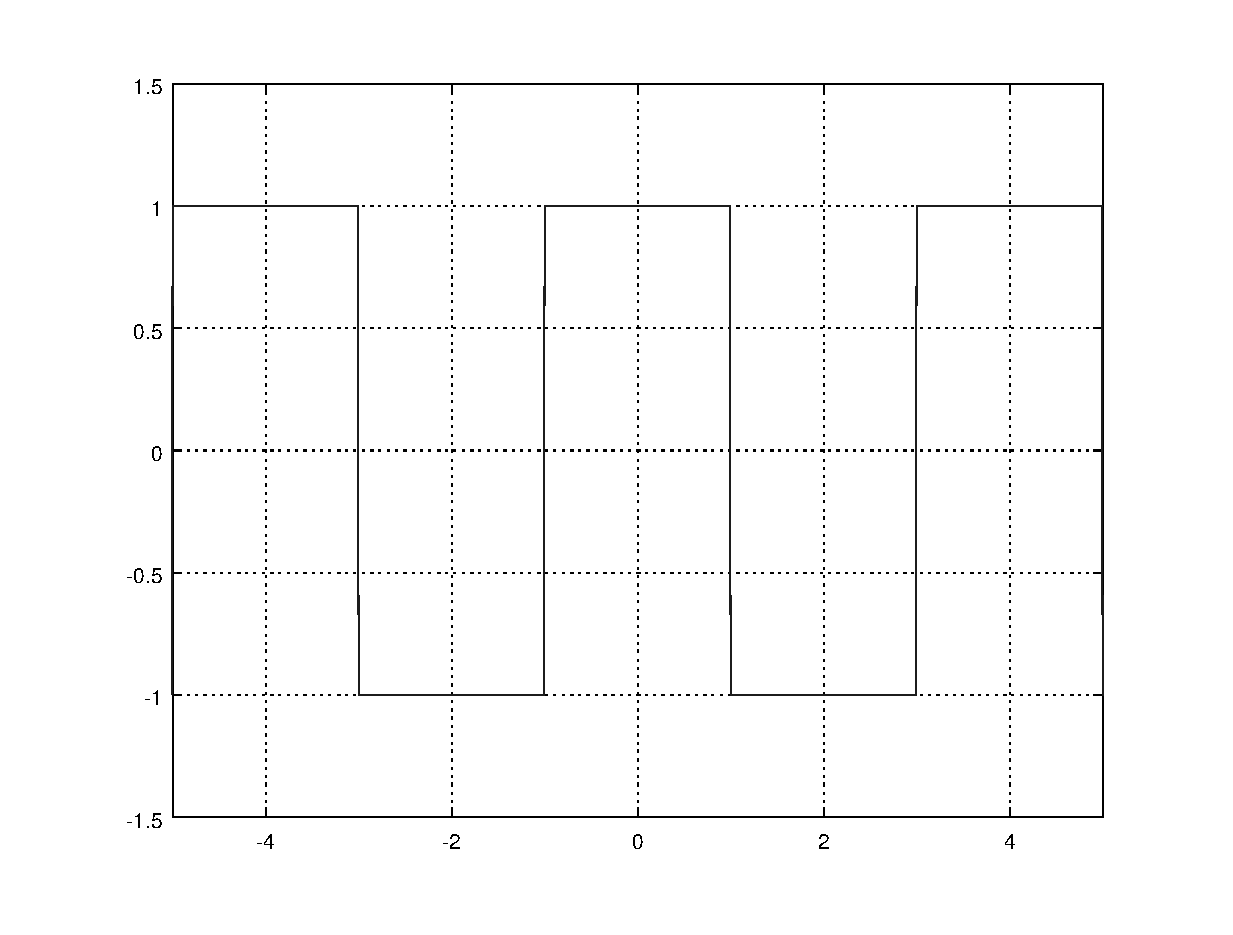
\includegraphics[width=\linewidth]{ej5}
            \caption{$x(t)$}
            \label{fig:Ej5}
        \end{center}
    \end{figure}
\end{multicols}
\begin{itemize}
    \item[a)] Grafique $m(t)$.
    \begin{figure}[H]
        \begin{center}
            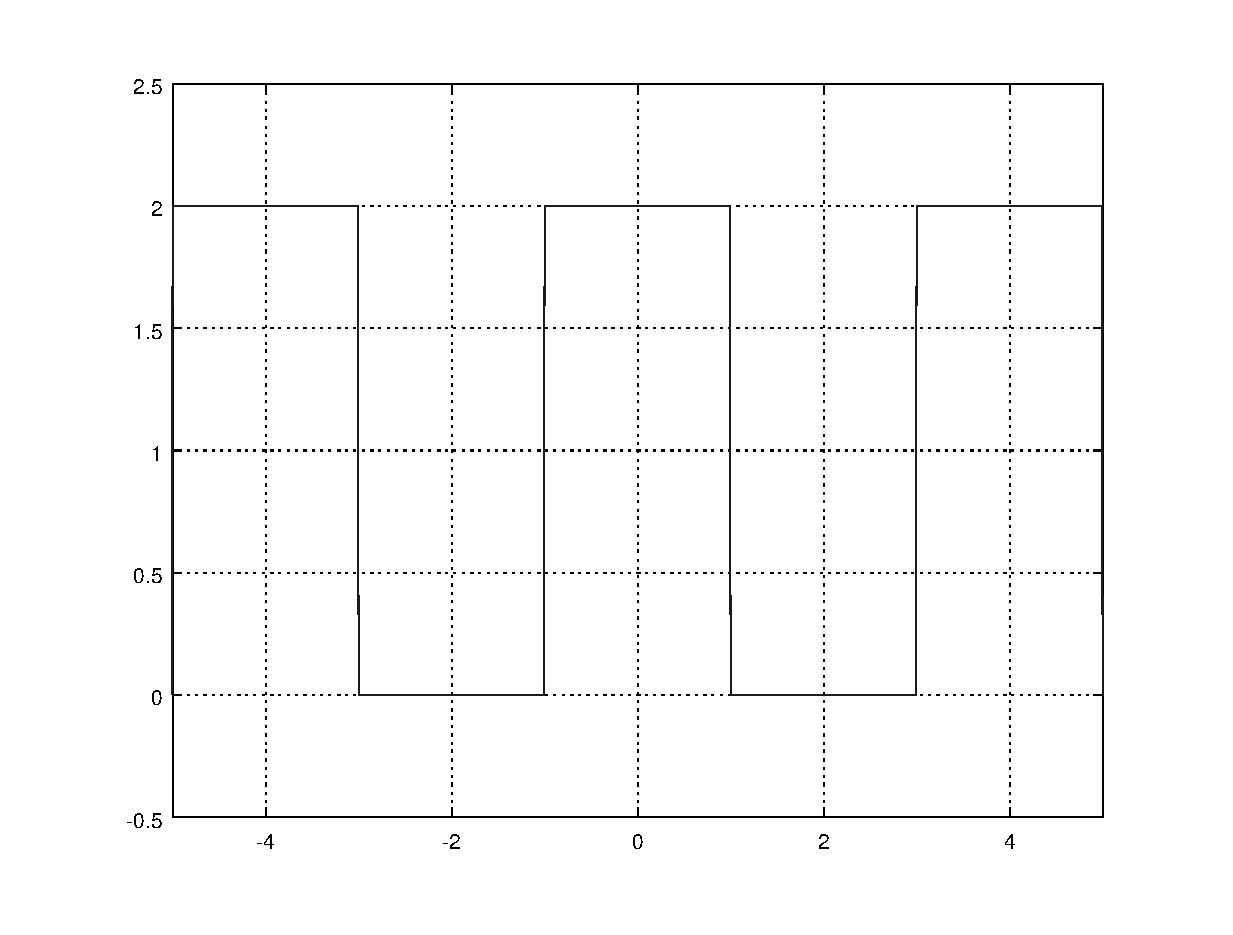
\includegraphics[width = 0.7\linewidth]{mt.eps}
            \caption{$m(t)$}
            \label{fig:mt}
        \end{center}
    \end{figure}
    Código en Matlab:
    \begin{lstlisting}
plot(t,1 + square(t./2*pi + pi/2));
axis([-5 5 -0.5 2.5]);grid;
    \end{lstlisting}
    \item[b)] Grafique el espectro de $m(t)$.
    \[ a_0 = \frac{1}{2} \qquad a_k = \frac{2}{k\pi}sen\left(\frac{\pi}{2}k\right) \]
\begin{multicols}{2}
    \begin{figure}[H]
        \begin{center}
            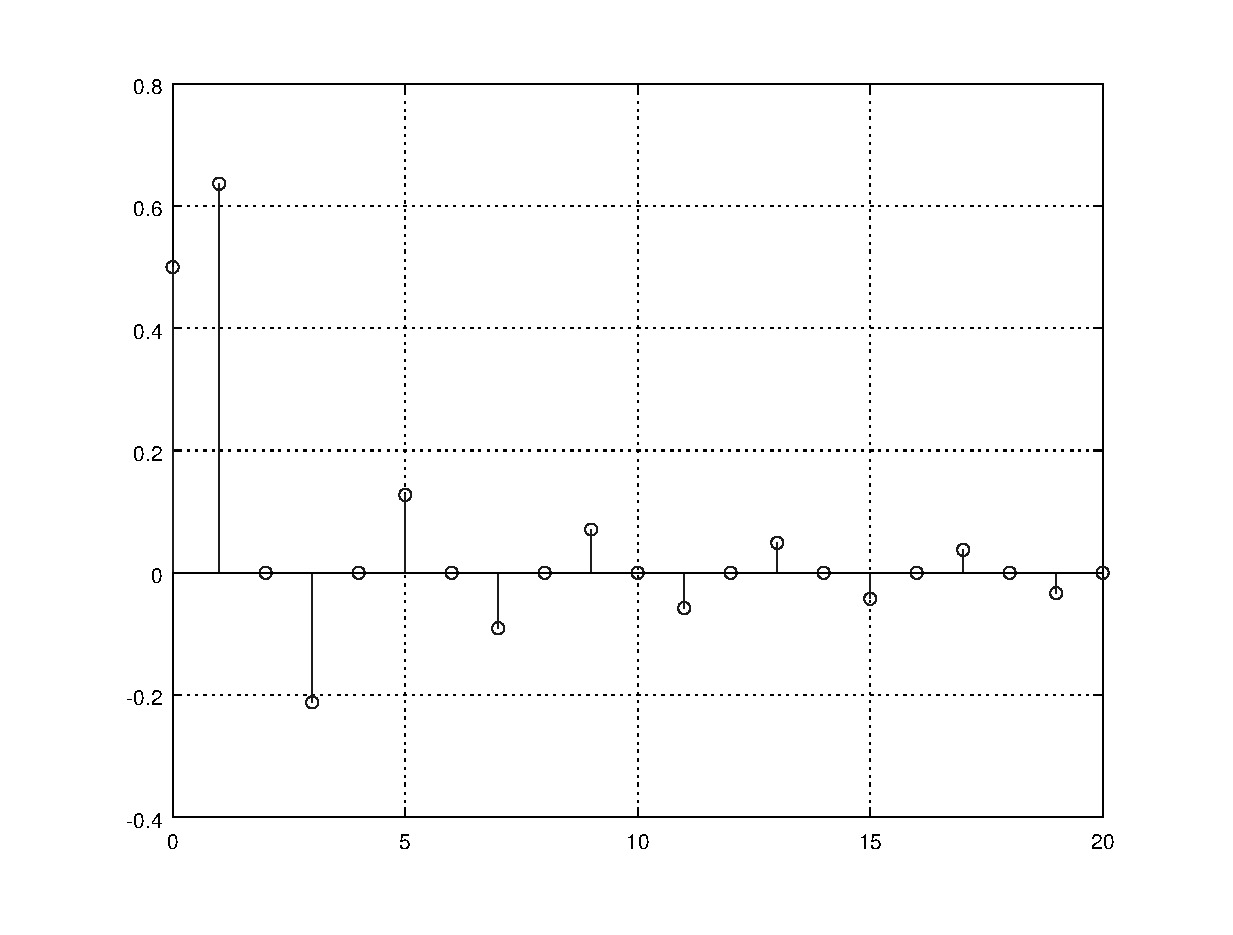
\includegraphics[width=\linewidth]{ak2}
            \caption{Espectro de la señal y código de Matlab}
            \label{fig:ak2}
        \end{center}
    \end{figure}
    \columnbreak
    \lstinputlisting{ak2.m}
    \begin{lstlisting}
stem(k,ak2(20));
    \end{lstlisting}
\end{multicols}
    \item[c)] Seleccione los filtros Butterwoth apropiados de manera que $y(t)= 1^a$ armónica y $y1(t) = 5^a$ armónica. \\
    \end{itemize}
    Para $y(t) \quad \omega_{c_1} = \frac{\pi}{3}, \quad \omega_{c_2} = \frac{2\pi}{3}$ \\  
    \[ H(z) = \frac{1.203s^4}{s^8 + 2.736s^7 + 12.52s^6 + 21.01s^5 + 46.49s^4 +46.07s^3 + 60.21s^2 +28.87s +23.14} \]
    \begin{lstlisting}
t=0:0.01:30;
[b a] = butter(4,[pi/3 2*pi/3],'s')
filtro = tf(b,a)
lsim(filtro,x4(50,t),t)
    \end{lstlisting}
    Para $y_1(t) \quad \omega_{c_1} = \frac{7\pi}{3}, \quad \omega_{c_2} = \frac{8\pi}{3}$
    \[ H(z) =  \frac{1.203s^4}{s^8 +2.736s^7 + 249.4s^6 + 507.1s^5 23090s^4 + 31140s^3 + 940500s^2 +633800s + 14220000} \]
    \begin{lstlisting}
t=0:0.01:30;
[b a] = butter(4,[7*pi/3 8*pi/3],'s')
filtro = tf(b,a)
lsim(filtro,x4(10,t),t)
    \end{lstlisting}

\end{document}
